\section{Allgemeines}

Um Anfragen mit SPARQL an RDF-basierte Datenbanken formulieren zu können muss zunächst eine gewisse Einstiegshürde überwunden werden. Selbst für weniger komplexe Anfragen müssen grundlegende Syntax und Vokabular der SPARQL vertraut sein.

Mit dem Graphical SPARQL Builder (GSB) soll diese Einstiegshürde gesenkt werden.
Dazu setzt der GSB auf eine graphische Repräsentation der Anfrage gegenüber einer rein textbasierten Anfrage in SPARQL.

Zum einen soll eine Anfrage möglichst intuitiv mithilfe einer graphischen Benutzeroberfläche erstellt werden können, zum anderen soll die Anfrage auch mit minimaler Vorkenntnis von RDF und SPARQL lesbar sein.

\section{Produktübersicht}

Abbildung~\ref{fig01} gibt eine Übersicht über die Eingliederung und
Nutzung des Graphical SPARQL Builder beim Einsatz des Tools im
Zusammenspiel mit beteiligten Personen und externen
Softwarekomponenten:

\begin{SCfigure}[20][!b]%
  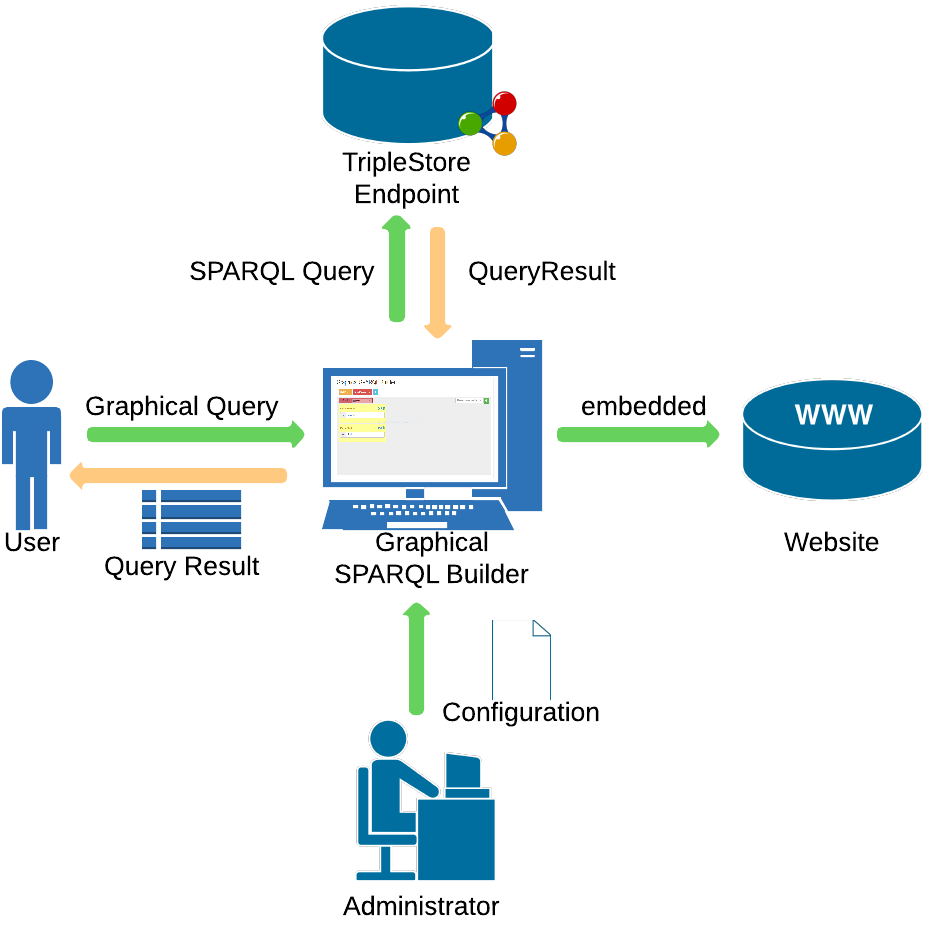
\includegraphics[width=.7\hsize]{Produktuebersicht2.png}
  \caption{Beziehung des GSB zu Anwender, Datenbank und Administration.}
  \label{fig01}
\end{SCfigure}

Im typischen Anwendungsfall möchte ein User (ohne SPARQL Kenntnisse)
eine Anfrage an eine RDF-basierte Datenbank stellen. 
Dazu stellt er sich die Anfrage grafisch im GSB zusammen und sendet
sie ab. Der GSB übersetzt die grafische Repräsentation der Anfrage
(zunächst in ein intern vordefiniertes JSON-Format und dann) in eine
semantisch und syntaktisch korrekte SPARQL-Anfrage. 
Das Tool sendet diese dann an einen vom Administrator eingestellten
SPARQL-Endpunkt eines TripleStores, von welchem das Anfrageergebnis
zurückgegeben wird. Der GSB leitet das Ergebnis an den User weiter.

Der Administrator hat die Möglichkeit über Konfigurationsdateien
diverse Einstellungen, wie Sprachwahl, Einschränkungen der
bereitgestellten Datenbank, Expertenansicht und zahlreiche
GUI-Anpassungen vorzunehmen.
Als Single-Page-Anwendung kann der GSB in bestehende Websites eingebettet werden.


\section{Grundsätzliche Struktur- und Entwurfsprinzipien}

Die Grundsätzliche Struktur des GSB ist im Komponentendiagramm
(Abb. \ref{fig02}) schematisch dargestellt.

%\begin{SCfigure}[20][htbp]%
\begin{figure}[h]%
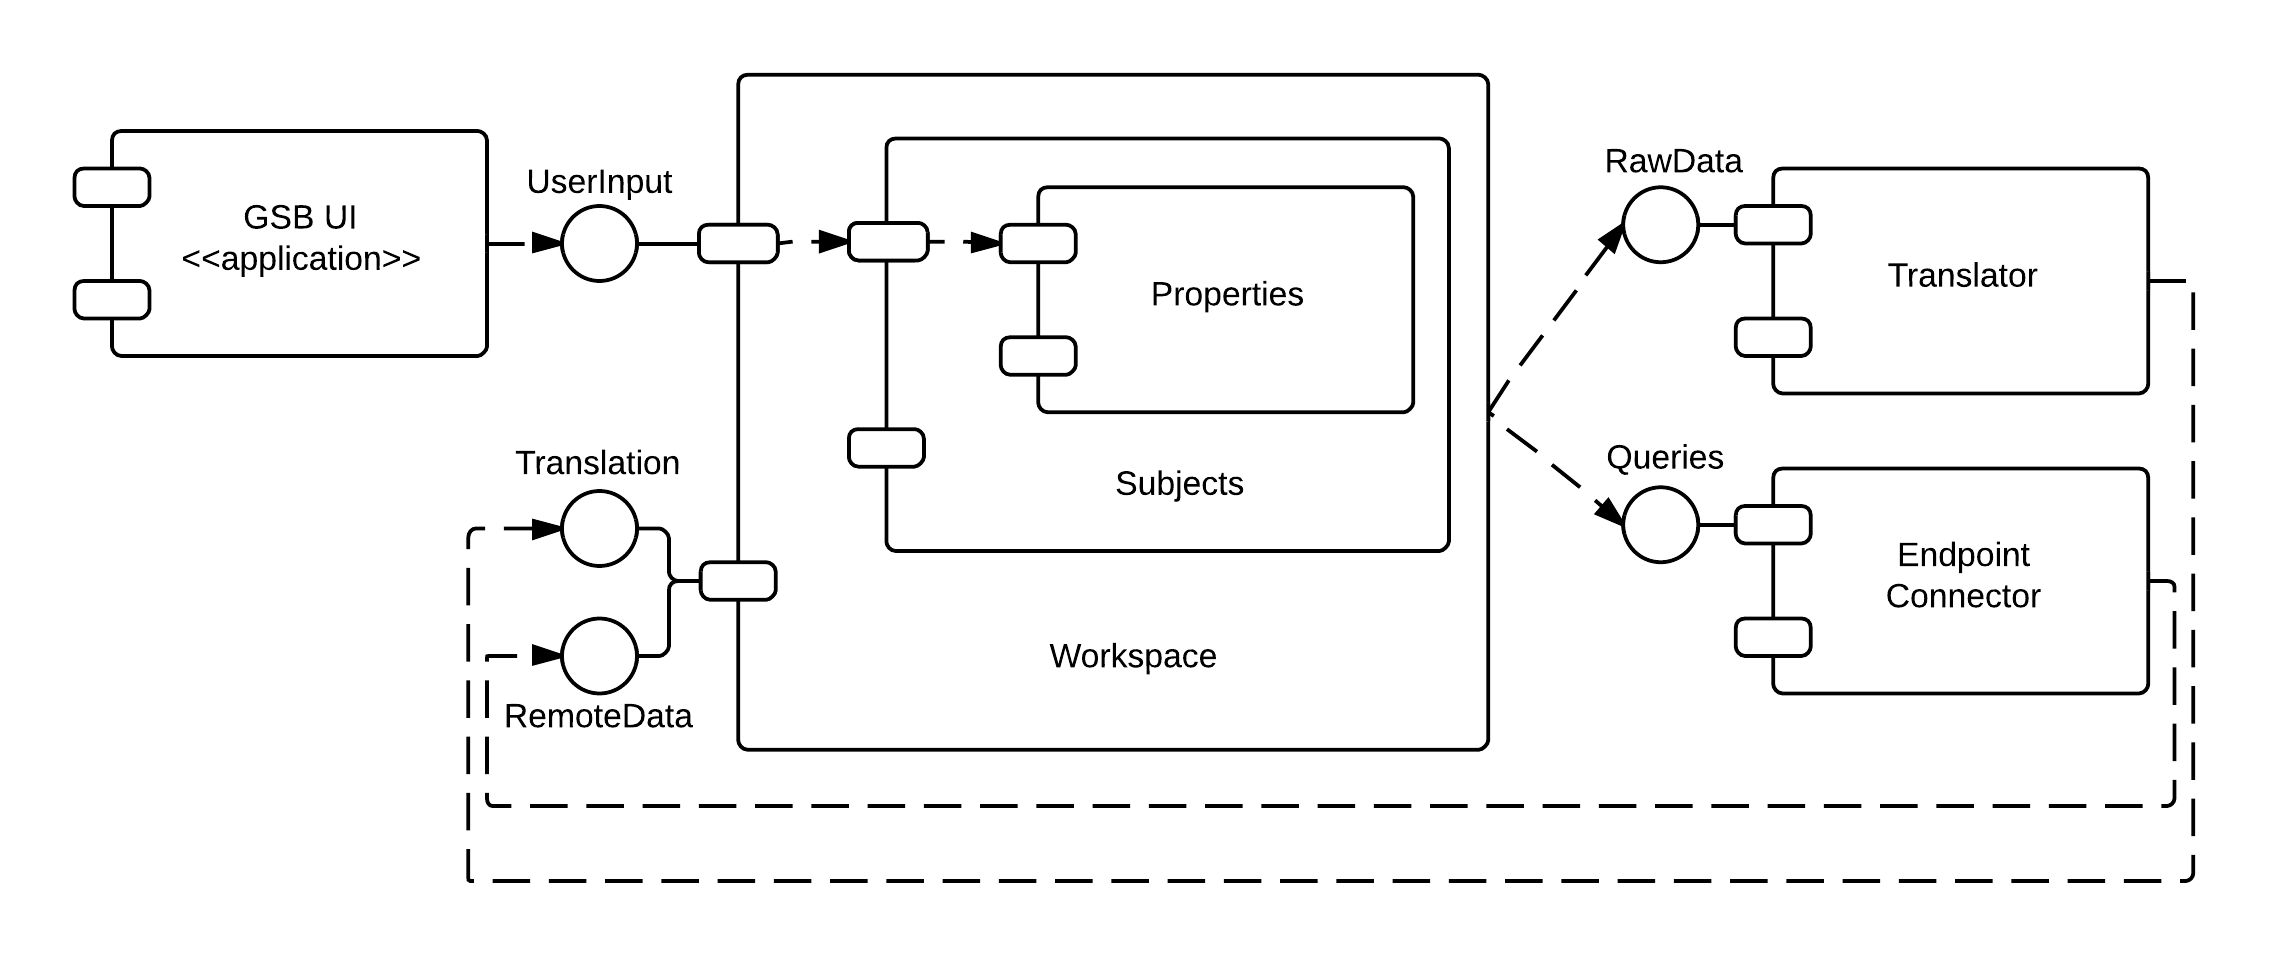
\includegraphics[width=\hsize]{Komponentendiagramm.png}
\caption{Komponentendiagramm des GSB.}
\label{fig02}
\end{figure}
%\end{SCfigure}


Es gibt die Komponente des User Interface (GSB UI), in welcher alle
Eingaben des Benutzers des Tools stattfinden. Diese werden in die
Komponente Workspace weitergeleitet und dort gegebenenfalls an die
Komponenten Subjects und deren Unterkomponente Properties
weitergeleitet. Um dies zu verdeutlichen, hier drei Beispiele:
\begin{enumerate}
\item Der Nutzer setzt eine Übersetzung eines GSBL-Wortes in Gang, dies betrifft die Komponente \glqq Workspace\glqq
\item Der Nutzer ändert den Alias eines Subjekts, dies würde über die Workspace-Komponente zu der Subjects-Komponente weitergereicht werden.
\item Der Nutzer ändert die Sichtbarkeit einer Eigenschaft, dies würde über die Workspace-Komponente zu der Subjects-Komponente zum Ziel, der Properties-Komponente, weitergereicht werden.
\end{enumerate}
Die Workspace-Komponente steht in Verbindung mit der
Translator-Komponente, welche für die Übersetzung der erstellten
Rohdaten zu JSON bzw. SPARQL zuständig ist und die Ergebnisse zurück
zur Workspace-Komponente überträgt.
Ebenso gibt es eine Verbindung zur Endpoint-Connector-Komponente, die die Kommunikation mit einem Endpoint übernimmt. Es können Anfragen gesendet und Ergebnisse empfangen werden.



\section{Struktur- und Entwurfsprinzipien einzelner Pakete}

\subsection*{User Interface}

Bei der Hauptversion des Projekts besteht das Userinterface aus dem
Workspace, der die graphisch konstruierte Abfrage beinhaltet, dem Feld
in dem nach dem Drücken des \glqq Build Query\grqq -Buttons die Übersetzung der
Anfrage in JSON und in SPARQL zu sehen ist.
Im Workspace befindet sich der Hinzufüge-Button für Subjekte sowie ein LIST ALL Objekt.
Ein weiterer Button ermöglicht das Speichern der Anfrage im
JSON-Format.

Das Laden einer gespeicherten Anfrage wird dem Nutzer durch
Drag\,\&\,Drop ermöglicht.
Standardmäßig werden zu Beginn zwei Subjekte (Mensch und Stadt) in den
Workspace geladen.
Subjekte und Properties sind durch Icons entfernbar sowie in der Abfrage anzeigbar.
Ein Link über dem SPARQL-Result-Feld ermöglicht zusätzlich das Anzeigen des Ergebnisses der übersetzten Anfrage, welches zurückgegeben wird nachdem die Anfrage an einen Endpunkt geschickt wurde.

\subsection*{Workspace}

Der Workspace umfasst die Sammlung von Subjekten, deren Properties und den Startpunkt sowie die Verbindungen (Linien) zwischen Subjekten und dem Startpunkt und einem Subjekt.

\subsection*{Subjects}

Subjects können durch die Icons entfernt (Papierkorb), in der Anfrage
aus-/eingeblendet (Auge) und hinzugefügt (Plus-Symbol) werden. Die
Properties eines Subjects sind ausblendbar.

Subjects sind Instanzen die mit den jeweiligen \glqq extern\grqq -Properties
Verbindungen untereinander aufbauen und Subject-interne Properties
sammeln. Miteinander verknüpfte Subjects sind durch Linien
verbunden. Subjects können durch Drag\,\&\,Drop auf dem Workspace
verschoben werden. Sie bilden den grundsätzlichen Anhaltspunkt für die
Übersetzung. (siehe {\sffamily\bfseries Translator})

\subsection*{Properties}

\Hack{\enlargethispage{1.5\baselineskip}}
Properties können durch die Icons entfernt (Papierkorb), in der Anfrage aus-/eingeblendet (Auge) und hinzugefügt (Add-Button beim Subject-Mouseover) werden.
Sie stellen über eine Auswahl im Drop-Down Menü eines Subjects Verbindungen zwischen Subjects her. Properties sind im Vergleich zum Vorprojekt um arithmetische Operatoren (\verb-+-, \verb+-+, \verb+*+, \verb+/+, \verb+COUNT+, \verb+MAX+, \verb+MIN+, \verb+SUM+) erweitert.

\subsection*{Translator}

Die Translator-Funktion ist auch in der Hauptversion des Projekts
zweigeteilt. Eine Übersetzung liefert auf Basis der im Workspace
zusammengestellten graphischen Anfrage (in GSBL) eine Abfrage im
JSON-Format und eine weitere Übersetzung von JSON in SPARQL wird
danach durchgeführt.

Die Translation wird durch Klick auf den Button \glqq Build Query\grqq gestartet und das Ergebnis wird in den unteren Feldern (JSON- und SPARQL-Resultat) angezeigt.
Algorithmisch betrachtet beginnt die Übersetzung bei dem mit dem
Startpunkt verknüpften Subject und übersetzt dann rekursiv alle damit
verknüpften Subjects und deren Properties, sodass nicht verknüpfte
Subjects ignoriert werden.


\subsection*{Endpunkt-Anbindung}

Anstatt wie im Vorprojekt lokal gespeicherte MockupDaten zu nutzen,
wird im Hauptprojekt auf einen SPARQL-Endpunkt zugegriffen. Die
Auswahl gegebener Subjekte beim Hinzufügen, deren mögliche
Eigenschaften sowie die LinkedSubjects werden am Endpunkt abgefragt
und dann im UI zur Verfügung gestellt. Je nach Vorankommen der
Projektarbeiten wird ein mehr oder weniger aufwendiger Cache
realisiert um starke Redundanz bei den Anfragen an den Endpunkt zu
vermeiden.

\section{Datenmodell}

Die Grundbausteine des RDF-Datenmodells sind Ressourcen, Eigenschaften und Aussagen. Durch diese ist es möglich RDF Ausdrücke syntaxfrei darzustellen.

\subsection*{Ressource}

Eine Ressource wird mit RDF Ausdrücken beschrieben. Folglich muss diese durch eine URI (Universal Resource Identifier) referenzierbar sein und eindeutig von dieser identifiziert werden können.

\subsection*{Eigenschaft}

Eigenschaften sind die Attribute von Ressourcen. Im Datenmodell legen sie die erlaubten Werte, den Typ und die Relation der Ressource zu anderen Ressourcen fest.

\subsection*{Aussage}

Eine Ressource, kombiniert mit ihrer Eigenschaft und den Wert, den die Eigenschaft dieser Ressource hat, nennt man \glqq Aussage\grqq. D.h. eine Aussage besteht aus Subjekt-Prädikat-Objekt (Ressource-Eigenschaft-Wert).

\Hack{\pagebreak}


\subsection*{Beispiel}
%\Hack{\enlargethispage{\baselineskip}}
\begin{SCfigure}[20][!h]%
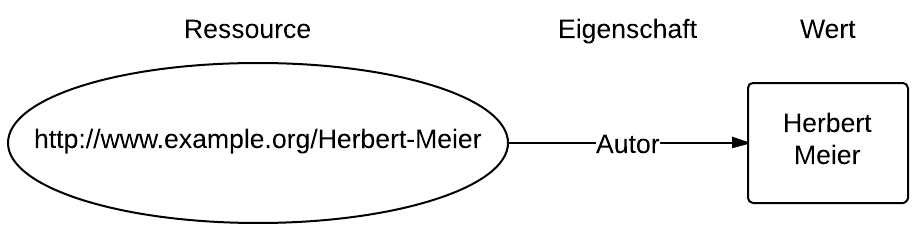
\includegraphics[width=.7\hsize]{datenmodell.png}
\caption{Beispiel eines RDF Tripels.}\label{fig03}
\end{SCfigure}
\begin{SCtable}[20][!h]%
\caption{Beispiel eines RDF Tripels.}
\begin{tabular}{l l}\toprule
Aussage  & Der Autor der Ressource ist Herbert Meier \\\midrule
Subjekt  & \url{http://www.example.org/Herbert-Meier} \\
Prädikat & Autor \\
Objekt   & \glqq Herbert Meier\grqq \\\bottomrule
\end{tabular}
\end{SCtable}

\subsection*{Repräsentation in JSON}

Im GSB werden die Informationen der graphischen, zu einer Anfrage
zusammengestellten Elemente zunächst innerhalb eines JSON-Objekts
gespeichert.
Dies soll einen Import/Export der gebauten Anfragen ermöglichen, und
dient gleichzeitig als Eingabeparameter für den Übersetzer, welcher
das JSON-Objekt schließlich in eine gültige SPARQL-Anfrage wandelt.
Die Erstellung dieses Objekts wird dabei erheblich durch die objektorientierte Repräsentation der grafischen Elemente erleichtert.

Im JSON-Objekt werden alle wichtigen Parameter einer Anfrage
festgehalten:
\begin{itemize}
\item In einem START-Objekt werden zunächst Typ und Linkpartner des
Startpunktes gespeichert. 
\item Danach folgen in einem SUBJECTS-Array alle vorkommenden
  Subjekte, mit wichtigen Variablen wie URI, Alias, Typ, etc. 
\item Innerhalb eines Subjekts befindet sich schließlich das properties-Array, in dem alle für das Subjekt gewählten Eigenschaften, inklusive deren eigene Parameter (Alias, URI etc.), zu finden sind.
\end{itemize}

Die Vorlage für ein solches JSON-Objekt befindet sich in Anhang~\ref{json}.

\section{Testkonzept}

Für die Qualitätssicherung dieses Projekt werden zunächst einzelne
Komponenten auf ihre \glqq interne Qualität\glqq hin getestet, und schließlich
die Zusammenführung dieser. Für Komponenten- bzw Integrationstests
bietet das für den GSB genutzte Framework AngularJS dabei bereits
eigene, potente Werkzeuge an~\cite{ajsut}. Diese erlauben losgelößte Tests
einzelner Funktionen, ohne etwa von der Antwort eines XMLHttpRequest
anhängig sein und diesen stattdessen zu simulieren. Für Systemtests
dagegen bietet Protractor ein Testframework für
AngularJS-Applikationen~\cite{prot}. Dabei kann die Anwendung direkt im
Browser getestet und mit ihr aus der Sicht eines Users interagiert
werden.

Besonders in den abschließenden Systemtest-Läufen sind identifizierte
Fehler zu dokumentieren, sowie, wenn möglich, deren Ursachen und
Bereinigung. Dadurch kann die Vermeidung ähnlicher Probleme
erleichtert werden, und Anhaltspunkte für die Suche mögliche
Fehlerquellen bereitgestellt werden.

Es soll außerdem ein besonderes Augenmerk auf Nutzungstests durch
Projekt-fremde User gelegt werden. Dadurch kann Feedback zu den für
den GSB essentiellen Aspekten Benutzbarkeit und Intuitivität gewonnen
werden, von Laien, die ihrerseits keine weitreichenden Erfahrungen mit
SPARQL haben und sich dadurch mit der Zielgruppe des Projekts
decken. Auch das Aufdecken möglicher Ausfälle bei falscher Benutzung
sind denkbar.
Im Besonderen betrifft dies die Mitarbeiter der Bibliotheca Albertina,
welche als mögliche Abnehmer des GSB bereits feststehen. Deren
Rückmeldungen sollen insofern stark gewichtet werden, da sie besonders
\glqq praxisnahe\glqq Probleme aufzeigen und Verbesserungsvorschläge liefern
könnten. Zu diesem Zweck ist auch ein regelmäßiges Treffen geplant.





%%% Local Variables: 
%%% mode: latex
%%% TeX-master: "main"
%%% End: 
